\hypertarget{Splits_8h}{
\section{Splits.h File Reference}
\label{Splits_8h}\index{Splits.h@{Splits.h}}
}


This graph shows which files directly or indirectly include this file:\nopagebreak
\begin{figure}[H]
\begin{center}
\leavevmode
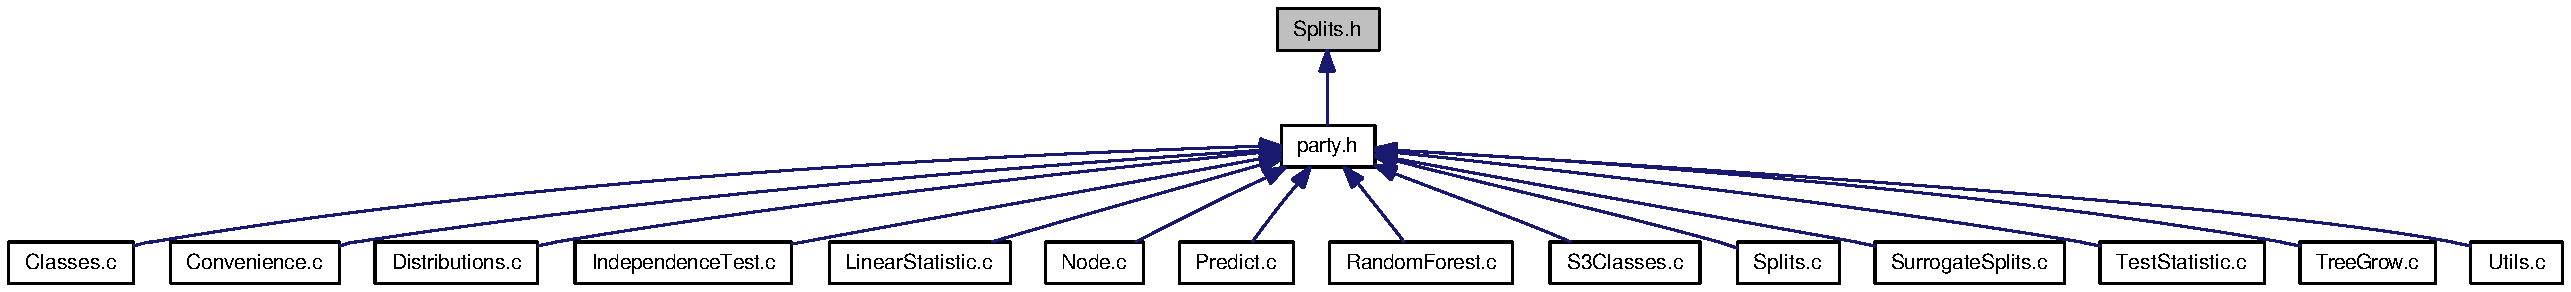
\includegraphics[width=420pt]{Splits_8h__dep__incl}
\end{center}
\end{figure}
\subsection*{Functions}
\begin{CompactItemize}
\item 
void \hyperlink{Splits_8h_00d4080fae6513962bd1e54ec9d476bc}{C\_\-split} (const double $\ast$x, int p, const double $\ast$y, int q, const double $\ast$weights, int n, const int $\ast$orderx, SEXP splitctrl, SEXP linexpcov2sample, SEXP expcovinf, double $\ast$cutpoint, double $\ast$maxstat, double $\ast$statistics)
\item 
void \hyperlink{Splits_8h_1b9f04a865d61c1c9757ba77bff49ab7}{C\_\-splitcategorical} (const int $\ast$codingx, int p, const double $\ast$y, int q, const double $\ast$weights, int n, double $\ast$standstat, SEXP splitctrl, SEXP linexpcov2sample, SEXP expcovinf, double $\ast$cutpoint, int $\ast$levelset, double $\ast$maxstat, double $\ast$statistics)
\end{CompactItemize}


\subsection{Function Documentation}
\hypertarget{Splits_8h_00d4080fae6513962bd1e54ec9d476bc}{
\index{Splits.h@{Splits.h}!C\_\-split@{C\_\-split}}
\index{C\_\-split@{C\_\-split}!Splits.h@{Splits.h}}
\subsubsection[C\_\-split]{\setlength{\rightskip}{0pt plus 5cm}void C\_\-split (const double $\ast$ {\em x}, \/  int {\em p}, \/  const double $\ast$ {\em y}, \/  int {\em q}, \/  const double $\ast$ {\em weights}, \/  int {\em n}, \/  const int $\ast$ {\em orderx}, \/  SEXP {\em splitctrl}, \/  SEXP {\em linexpcov2sample}, \/  SEXP {\em expcovinf}, \/  double $\ast$ {\em cutpoint}, \/  double $\ast$ {\em maxstat}, \/  double $\ast$ {\em statistics})}}
\label{Splits_8h_00d4080fae6513962bd1e54ec9d476bc}


Search for a cutpoint in a ordered variable x maximizing a two-sample statistic w.r.t. (the influence function of ) the response variable y. \begin{Desc}
\item[Parameters:]
\begin{description}
\item[{\em x}]raw numeric measurements \item[{\em p}]dimension of the transformation \item[{\em y}]values of the influence function \item[{\em q}]dimension of the influence function \item[{\em weights}]case weights \item[{\em n}]number of observations \item[{\em orderx}]the ordering of the transformations, i.e. R$>$ order(x) \item[{\em splitctrl}]an object of class `SplitControl' \item[{\em linexpcov2sample}]an (uninitialized) object of class `LinStatExpectCovar' with p = 1 \item[{\em expcovinf}]an initialized object of class `ExpectCovarInfluence' \item[{\em cutpoint}]return value; pointer to a double for the cutpoint in x \item[{\em maxstat}]return value; pointer to a double for the maximal test statistic \item[{\em statistics}]return value; pointer to a n-dim double for the statistics \end{description}
\end{Desc}


Definition at line 33 of file Splits.c.

References get\_\-minbucket(), get\_\-minprob(), get\_\-tol(), PL2\_\-covarianceSym, PL2\_\-expectationSym, PL2\_\-linearstatisticSym, and PL2\_\-sumweightsSym.

Referenced by C\_\-Node(), C\_\-splitcategorical(), C\_\-surrogates(), and R\_\-split().

Here is the call graph for this function:\nopagebreak
\begin{figure}[H]
\begin{center}
\leavevmode
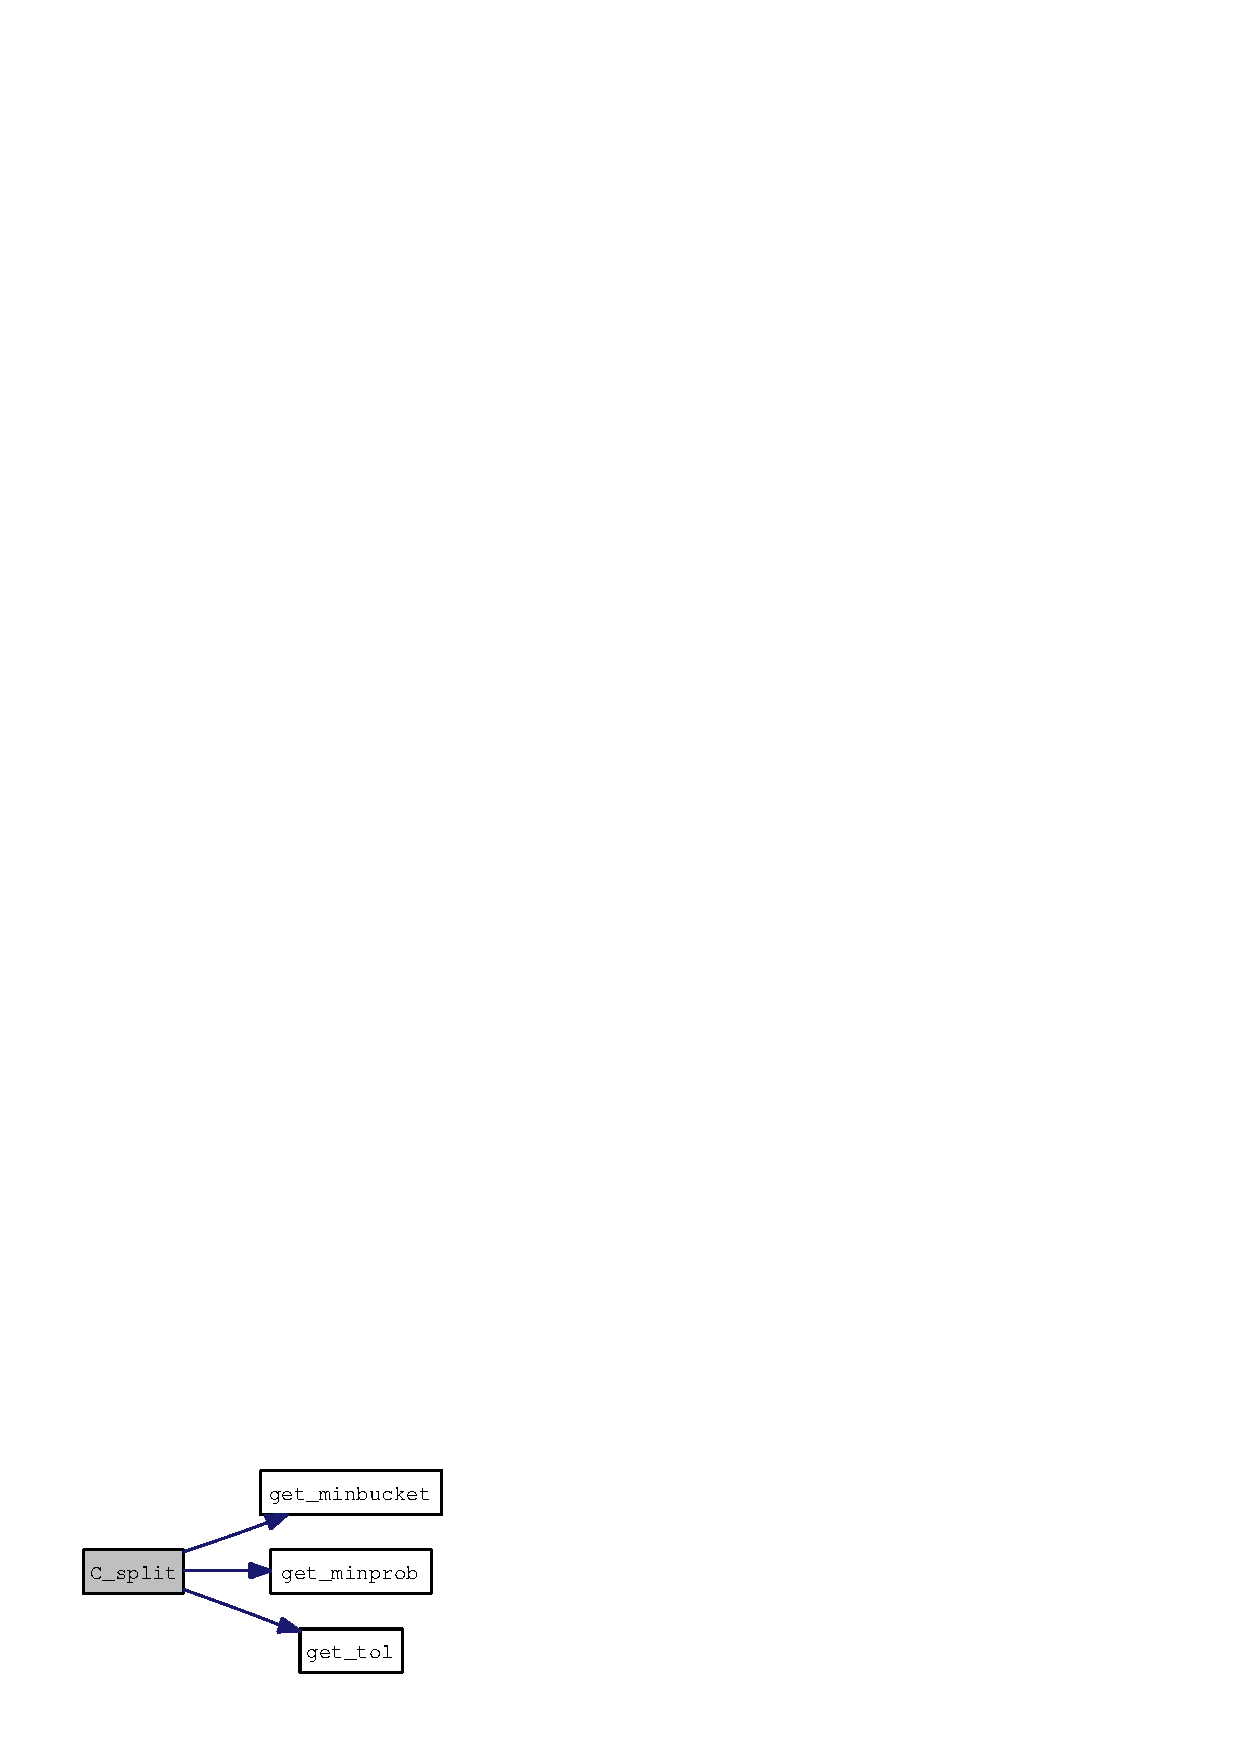
\includegraphics[width=103pt]{Splits_8h_00d4080fae6513962bd1e54ec9d476bc_cgraph}
\end{center}
\end{figure}
\hypertarget{Splits_8h_1b9f04a865d61c1c9757ba77bff49ab7}{
\index{Splits.h@{Splits.h}!C\_\-splitcategorical@{C\_\-splitcategorical}}
\index{C\_\-splitcategorical@{C\_\-splitcategorical}!Splits.h@{Splits.h}}
\subsubsection[C\_\-splitcategorical]{\setlength{\rightskip}{0pt plus 5cm}void C\_\-splitcategorical (const int $\ast$ {\em codingx}, \/  int {\em p}, \/  const double $\ast$ {\em y}, \/  int {\em q}, \/  const double $\ast$ {\em weights}, \/  int {\em n}, \/  double $\ast$ {\em standstat}, \/  SEXP {\em splitctrl}, \/  SEXP {\em linexpcov2sample}, \/  SEXP {\em expcovinf}, \/  double $\ast$ {\em cutpoint}, \/  int $\ast$ {\em levelset}, \/  double $\ast$ {\em maxstat}, \/  double $\ast$ {\em statistics})}}
\label{Splits_8h_1b9f04a865d61c1c9757ba77bff49ab7}


Search for a cutpoint in a unordered factor x maximizing a two-sample statistic w.r.t. (the influence function of ) the response variable y. \begin{Desc}
\item[Parameters:]
\begin{description}
\item[{\em codingx}]the coding of x, i.e. as.numeric(x) \item[{\em p}]dimension of the transformation \item[{\em y}]values of the influence function \item[{\em q}]dimension of the influence function \item[{\em weights}]case weights \item[{\em n}]number of observations \item[{\em codingx}]the coding of x, i.e. as.numeric(x) \item[{\em standstat}]the vector of the standardized statistics for x, y, weights \item[{\em splitctrl}]an object of class `SplitControl' \item[{\em linexpcov2sample}]an (uninitialized) object of class `LinStatExpectCovar' with p = 1 \item[{\em expcovinf}]an initialized object of class `ExpectCovarInfluence' \item[{\em cutpoint}]return value; pointer to a double for the cutpoint in x \item[{\em levelset}]return value; pointer to a p-dim 0/1 integer \item[{\em maxstat}]return value; pointer to a double for the maximal test statistic \item[{\em statistics}]return value; pointer to a n-dim double for the statistics \end{description}
\end{Desc}


Definition at line 217 of file Splits.c.

References C\_\-split(), and get\_\-tol().

Referenced by C\_\-Node(), and R\_\-splitcategorical().

Here is the call graph for this function:\nopagebreak
\begin{figure}[H]
\begin{center}
\leavevmode
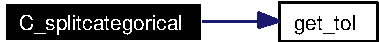
\includegraphics[width=168pt]{Splits_8h_1b9f04a865d61c1c9757ba77bff49ab7_cgraph}
\end{center}
\end{figure}
